%-------------------------------------------------
%	Version: 0.0
%	fecha de entrega 6 febrero 2021
%
%-------------------------------------------------

\documentclass[11pt]{report}

%packages
\usepackage{graphicx}
\usepackage{subcaption}

\usepackage[utf8]{inputenc}
\usepackage[spanish, es-nodecimaldot]{babel}
\usepackage{setspace}
\usepackage{ragged2e}

\usepackage{amsmath}
\usepackage{amsthm}
\usepackage{amssymb}
\usepackage{mathtools}
\usepackage{siunitx}
\usepackage[thinc]{esdiff} %derivadas faciles
\usepackage{physics} %algunos simbolos de derivadas

%path donde se encuentran las imagenes
\graphicspath{ {./figuras/} }

%---------------------------------------------------------------
%ABREVIACIONES DE COMANDOS
%---------------------------------------------------------------

\theoremstyle{plain}
\newtheorem{thm}{Teorema}[chapter] % reset theorem numbering for each chapter

\theoremstyle{definition}
\newtheorem{defn}[thm]{Definición} % definition numbers are dependent on theorem numbers
\newtheorem{exmp}[thm]{Ejemplo} % same for example numbers

\newcommand{\chaptercontent}{
\section{Basics}
\begin{defn}Here is a new definition.\end{defn}
\begin{thm}Here is a new theorem.\end{thm}
\begin{thm}Here is a new theorem.\end{thm}
\begin{exmp}Here is a good example.\end{exmp}
\subsection{Some tips}
\begin{defn}Here is a new definition.\end{defn}
\section{Advanced stuff}
\begin{defn}Here is a new definition.\end{defn}
\subsection{Warnings}
\begin{defn}Here is a new definition.\end{defn}
}

\usepackage{biblatex}
%\addbibresource{Tarea1.bib}

\begin{document}

\begin{titlepage}
\title{Examen_Caos}

%-------------------------------------------------
%PORTADA
%-------------------------------------------------

	\centering
	{\scshape\LARGE Universidad Autónoma de Yucatán  \\ Facultad de ingeniería\par}
	\vspace{1cm}
	{\scshape\Large Introducción al Caos\par}
	\vspace{1.5cm}
	{\huge\bfseries Examen 3\par}
	\vspace{0.7cm}
	{\begin{figure}[!h]
	\centering
    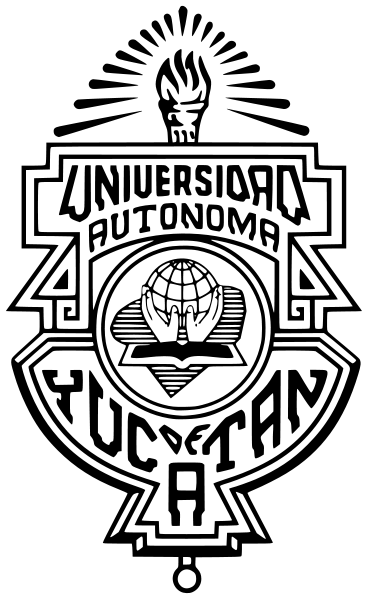
\includegraphics[scale=0.3]{UADY.png}
	\end{figure}}
	\vspace{0.7cm}
	{\Large\itshape Erick Al. Casanova Cortés\par}
	{\Large\itshape Matricula: 15014866\par}
	\vfill
	{\scshape\Large Docente\par
	Dr. Cesar Acosta\par}
	\vfill
	{\Large{\bfseries Fecha de entrega: 6 Febrero 2021} }

	\vfill
	
\end{titlepage}

%-------------------------------------------------
%Inicio del documento
%-------------------------------------------------

\tableofcontents

%-------------------------------------------------
%Primer Ejercicio
%-------------------------------------------------
\section{Primer ejercicio}
\textit{Dada la función del espacio de fase $f(x) = x+cx^2+x^3+3$, halle el diagrama de bifurcación, seleccionando de modo adecuado el rango de validez del parámetro "$c$", así como el rango de validez de "$x$". Establezca los puntos en donde se daban las bifurcaciones (puntos de silla de montar), así como las ventanas (rango entre dos puntos de silla de montar).}\\

\begin{figure}[!h] %FUNCION
	\centering
	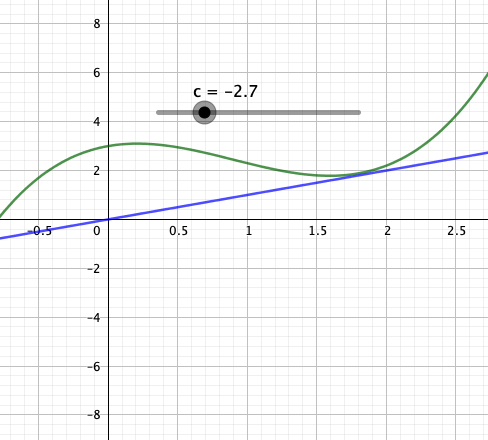
\includegraphics[scale=0.3]{caos_1_1.png}
	\caption{Función $f(x)$ con valor $c$ que genera un punto silla de montar}
	\label{fig:Eje1_1}
\end{figure}

Lo primero que se hizo fue graficar en geogebra la función $f(x)$, generando un deslizador $c$ para probar con distintos valores hasta encontrar uno que nos genere un punto de silla de montar. Este valor fue cercano a $c=-2.7$ como podemos apreciar en la figura \ref{fig:Eje1_1}



\begin{figure}[!h] %DIFURCACION
	\centering
	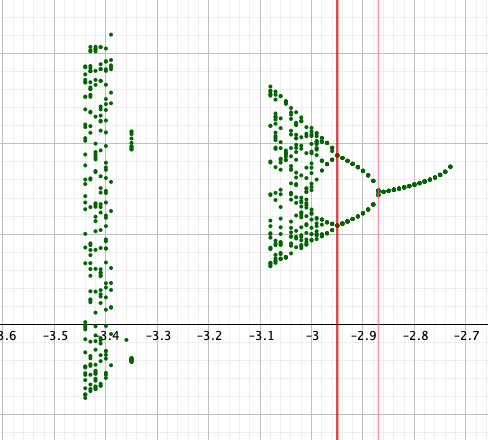
\includegraphics[scale=0.3]{caos_1_2.png}
	\caption{Diagrama de bifurcación}
	\label{fig:Eje1_2}
\end{figure}

Igual podemos apreciar que dicho punto de silla de montar se encuentra en $x\sim 1.72$. Ahora, para realizar el diagrama de difamación se tuvo que hacer un rango que incluya los valores de $c$, se optó por usar el rango $-4\leq c \leq-2$, y se optó por un rango en $x$ de $1\leq x \leq 3$, ya que dentro de este rango se encuentra el valor de $x$ que vimos anteriormente.

Se realizó una secuencia de puntos con el comando
\begin{verbatim}
	Sequence(Sequence((c, Iteration(x + c x^2 + x^3 + 3, p, 100)),
	 c, -4, -2, 0.01), p, 1, 3, 0.1)
\end{verbatim}
Cuyo resultado se puede ver en la figura \ref{fig:Eje1_2}


\begin{figure}[!h] %ZOOM
	\centering
	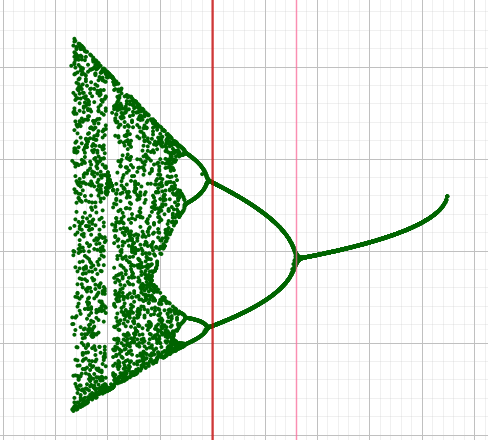
\includegraphics[scale=0.3]{caos_1_3.png}
	\caption{Vista aumentada de la región}
	\label{fig:Eje1_3}
\end{figure}

Igual se puede apreciar en la figura \ref{fig:Eje1_2} dos rectas, esas rectas están ubicados en los puntos de bifurcación del diagrama, ambas fueron aproximadas con dos deslizadores con el fin de tener una precisión mayor a solo ubicarlas, las rectas se encuentran en $x=-2.95$ y en $x=-2.87$. Por lo que la distancia entre ambas bifurcaciones puede ser calculada como:

\begin{align*}
	d &\sim |-2.95-(-2.87)|\\
	&\sim 0.08
\end{align*}


También se puede apreciar de mejor manera el diagrama de bifurcación en la figura \ref{fig:Eje1_3}, en esta parte se le hizo un aumento a la gráfica donde se encuentran las bifurcacinoes


%-------------------------------------------------
%Segundo ejercicio
%-------------------------------------------------
\section{Segundo ejercicio}
\textit{Dada la función del espacio de fase $f(x) = \lambda x(1-x)$, halle el diagrama de bifurcación, seleccionando de modo adecuado el rango de validez del parámetro "$\lambda$", así como el rango de validez de "$x$". Establezca los puntos en donde se dan las bifurcaciones (puntos de silla de montar), así como las ventanas (rango entre dos puntos de silla de montar)}

\begin{figure}[!h] %FUNCION
	\centering
	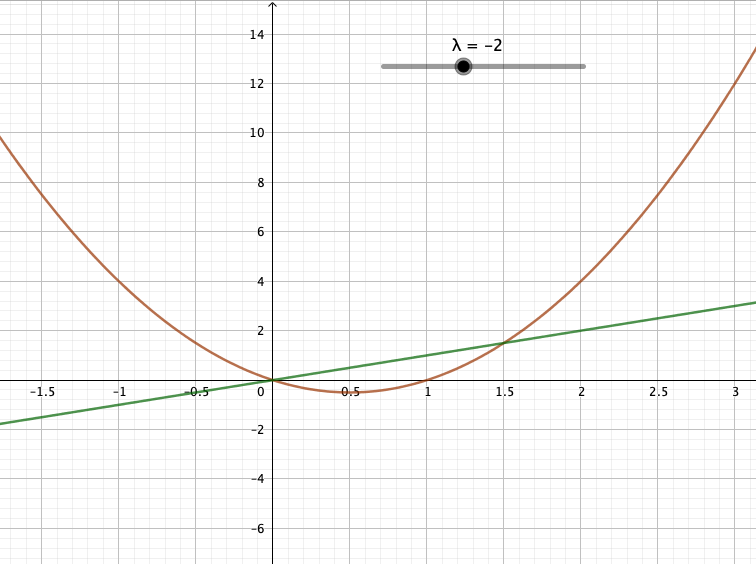
\includegraphics[scale=0.3]{caos_2_1.png}
	\caption{Función $f(x)$ con $\lambda = -2$}
	\label{fig:Eje2_1}
\end{figure}

Como en el anterior ejercicio se graficó la función $f(x)$ en geogebra. Una vez analizado el comportamiento de la función se encontró que en el rango de $-2 \leq \lambda \leq 4$ se encuentra el menor numero de puntos periódicos, y podemos ver que fuera de este intervalo, tanto como superior o inferior se genera una gran cantidad de puntos periódicos, lo cual se ve más adelante. En la figura \ref{fig:Eje2_1} se puede ver la gráfica de la función para un $\lambda = -2$, la cual se encuentra justo en el límite del intervalo propuesto, igual que el ejercicio anterior se uso el comando en geogbra para generar el diagrama de bifurcación, y se optó por valores de $-1 \leq x \leq 2$, esto por la magnitud de los puntos críticos obtenidos por la función en el rango de $\lambda$.\\


\begin{figure}[!h] %DIFURCACION 1
	\centering
	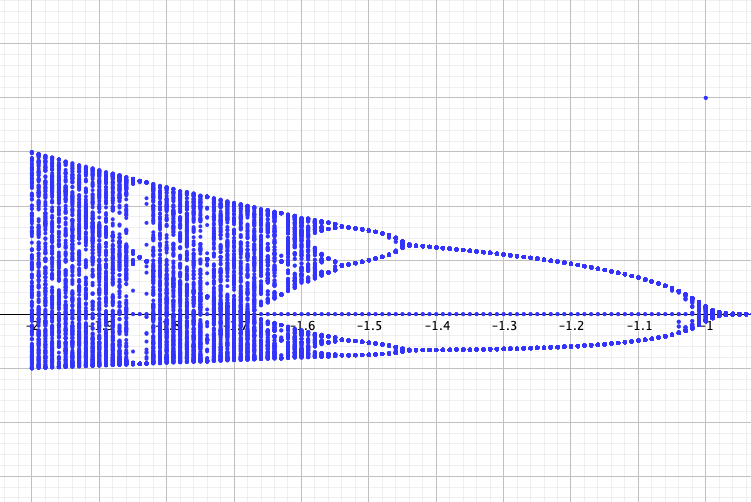
\includegraphics[scale=0.3]{caos_2_2.png}
	\caption{Diagrama de bifurcación de lado izquierdo}
	\label{fig:Eje2_2}
\end{figure}

Como se mencionó anteriormente, se puede ver que tiene un diagrama de ambos lados, analizando el del lado izquierdo, podemos apreciar su comportamiento en la figura \ref{fig:Eje2_2}. De igual manera podemos ver las rectas que pasan por los puntos en los que se bifurca en la figura \ref{fig:Eje2_3}

\begin{figure}[!h] %DIFURCACION 1 LINEAS
	\centering
	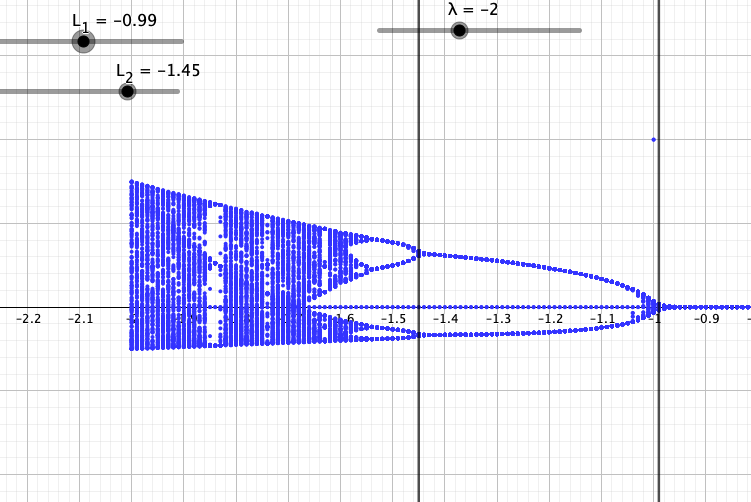
\includegraphics[scale=0.3]{caos_2_3.png}
	\caption{Diagrama de bifurcación con rectas}
	\label{fig:Eje2_3}
\end{figure}

\begin{figure}[!h] %DIFURCACION 2
	\centering
	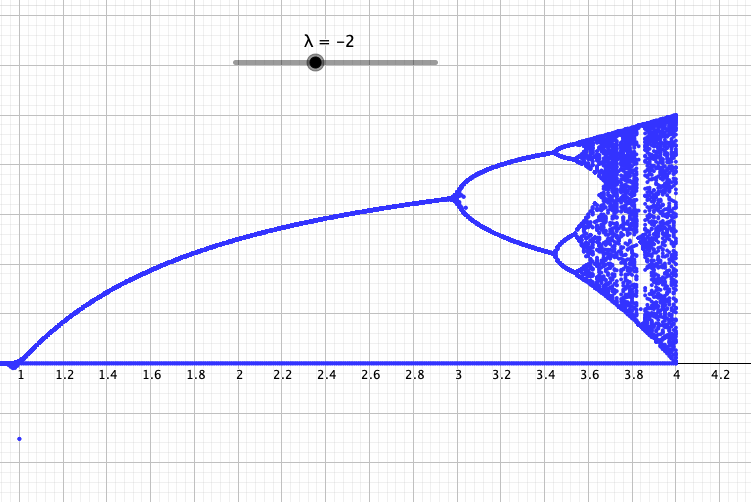
\includegraphics[scale=0.3]{caos_2_4.png}
	\caption{Diagrama de bifurcación de lado derecho}
	\label{fig:Eje2_4}
\end{figure}

\begin{figure}[!h] %DIFURCACION 2 LINEAS
	\centering
	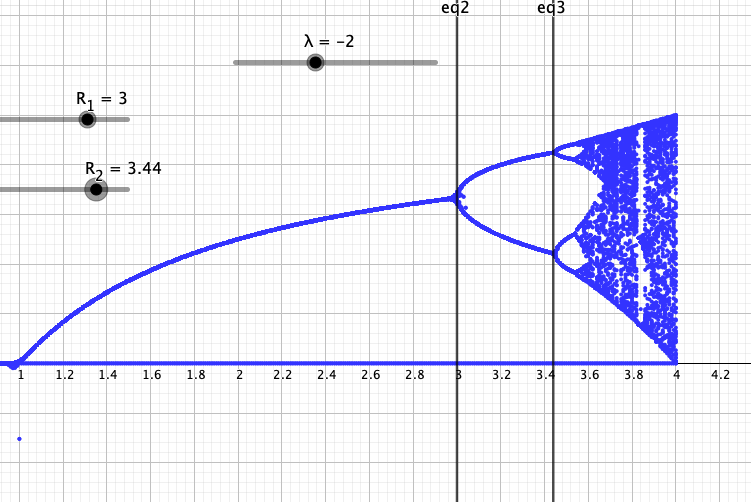
\includegraphics[scale=0.3]{caos_2_5.png}
	\caption{Diagrama de bifurcación con rectas}
	\label{fig:Eje2_5}
\end{figure}


El comportamiento del lado derecho se puede ver en la figura \ref{fig:Eje2_4}, así como las rectas que pasan por los puntos de bifurcación en la figura \ref{fig:Eje2_5}


Ahora calculando las distancias de las bifurcaciones 

\begin{align*}
	d_1 &\sim |-1.45-(-0.99)|\\
	&\sim 0.46
\end{align*}

\begin{align*}
	d_2 &\sim |2.99-3.44|\\
	&\sim 0.45
\end{align*}

Podemos ver que ambas distancias tienen magnitudes bastante similares
%-------------------------------------------------
%Tercer ejercicio
%-------------------------------------------------
\section{Tercer ejercicio}
\textit{Dada la función del espacio de fase $f(x) = c\sin(x)$, halle el diagrama de bifurcación para $0\leq c \leq 8\pi$, en donde el rango de validez de "$x$" es $0\leq x \leq 2\pi$. Establezca los puntos en donde se dan las bifurcaciones (puntos de silla de montar), así como las ventanas (rango entre dos puntos de silla de montar)}
%-------------------------------------------------
%Cuarto ejercicio
%-------------------------------------------------
\section{Cuarto ejercicio}
\textit{Dada la función del espacio de fase $f(X) = 5\cos(x)$, en donde el rango de validez de "$x$" es $-2\pi\leq x \leq 2\pi$. Establezca el itinerario para puntos de la quinta iteración y aplique a estos puntos la función $\sigma$ (mapa shift), muestre los resultados tanto en el sistema binario como en el sistema decimal.}
%-------------------------------------------------
%Final del documento
%-------------------------------------------------

\end{document}
